\chapter{Discussion}
Please tell more about conclusion and how to the next work of this study.

\section{Andri Fajar Sunandhar / 1164065}
\subsection{Teori}
\begin{enumerate}

\item Jelaskan kenapa file teks harus dilakukan tokenizer, dilengkapi dengan ilustrasi atau gambar.
	\par Tokenizer adalah untuk membuat vektor dari teks. File teks harus dilakukan tokenizer karena dengan memfungsikan tokenizer teks dapat divektorkan. Maka dari itu harus menginport tokenizer dari keras, sehingga teks yang telah telah divektorkan tersebut dapat terbaca pada Machine Learning. Ilustrasinya bisa dilihat pada gambar \ref{no1}.
	\begin{figure}[ht]
	\centerline{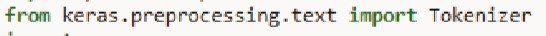
\includegraphics[width=0.5\textwidth]{figures/chapter7/no1.jpg}}
	\caption{Tokenizer}
	\label{no1}
	\end{figure}

\item Jelaskan konsep dasar K-Fold Cross Validation, dilengkapi dengan ilustrasi atau gambar.

\item Jelaskan apa maksudnya kode program for train, test in splits, dilengkapi dengan ilustrasi atau gambar

\item Jelaskan apa maksudnya kode program train\_content dan test\_content, dilengkapi dengan ilustrasi atau gambar.

\item Apa maksud dari fungsi tokenizer, dilengkapi dengan ilustrasi atau gambar.

\item Jelaskan apa maksud dari fungsi d\_train\_inputs dan d\_test\_inputs, dilengkapi dengan ilustrasi atau gambar.

\item 7.

\item Jelaskan apa maksud dari fungsi d\_train\_outputs dan d\_test\_outputs, dilengkapi dengan ilustrasi atau gambar.

\item Jelaskan apa maksud dari fungsi di listing 7.2 , Gambarkan ilustrasi Neural Networknya.

\item Jelaskan apa maksud dari fungsi di listing 7.3 .

\item Jelaskan apa itu Deep Learning.
	\par Deep Learning merupakan cabang dari Machine Learning atau bagian keluarga yang lebih luas dari method machine learning berdasarkan pada representasi data pembelajaran. Deep Learning menggunakan Deep Neural Network dalam menyelesaikan suatu masalah yang terjadi pada Machine Learning.

\item Jelaskan apa itu Deep Neural Network, dan apa bedanya dengan Deep Learning.
	\par Deep Neural Network atau DNN merupakan algoritma yang berbasis neural network yang digunakan untuk mengambil keputusan. Yang membedakan Deep Learning dengan  Deep Neural Network (DNN) adalah DNN merupakan algoritma yang digunakan pada Deep Learning, sedangkan Deep Learning merupakan model yang menggunakan algoritma DNN.

\item Jelaskan dengan ilustrasi gambar buatan sendiri bagaimana perhitungan algoritma konvolusi dengan ukuran stride (NPM mod3+1)x(NPM mod3+1) yang terdapat max pooling.

\end{enumerate}





\subsection{Praktek}
\begin{enumerate}
\item Jelaskan kode program pada blok \# In [1]. 

\item Jelaskan kode program pada blok \# In [2] .

\item Jelaskan kode program pada blok \# In [3] .

\item Jelaskan kode program pada blok \# In [4] .

\item Jelaskan kode program pada blok \# In [5] .

\item Jelaskan kode program pada blok \# In [6] .

\item Jelaskan kode program pada blok \# In [7] .

\item Jelaskan kode program pada blok \# In [8] .

\item Jelaskan kode program pada blok \# In [9] .

\item Jelaskan kode program pada blok \# In [10] .

\item Jelaskan kode program pada blok \# In [11] .

\item Jelaskan kode program pada blok \# In [12] .

\item Jelaskan kode program pada blok \# In [13] .

\item Jelaskan kode program pada blok \# In [14] .

\item Jelaskan kode program pada blok \# In [15] .

\item Jelaskan kode program pada blok \# In [16] .

\item Jelaskan kode program pada blok \# In [17] .

\item Jelaskan kode program pada blok \# In [18] .

\item Jelaskan kode program pada blok \# In [19] .

\item Jelaskan kode program pada blok \# In [20] .


\end{enumerate}





\subsection{Penanganan Error}
Dari praktek pemrograman yang dilakukan di modul ini, error yang kita dapatkan(hasil komputer sendiri) di dokumentasikan dan di selesaikan(nilai 5 per error yang ditangani. Untuk hari kedua):

\begin{enumerate}
	\item skrinsut error
		
		
	\item Tuliskan kode error dan jenis errornya
		\begin{enumerate}
		\item Kode Error  :
			\begin{itemize}
				\item Kode error : 
				\item Jenis error :
			\end{itemize}
		\end{enumerate}

	\item Solusi pemecahan masalah error
		
		
\end{enumerate}